%% Tex spellcheck = fr_FR
\thispagestyle{noheader}
\chapter*{Abstract} % No (numbered) toc entry with *

\tikz[remember picture,overlay] \node[shift={(4.165cm,-1.955cm)}]
at (current page.north west)
{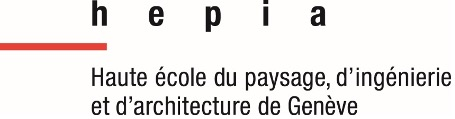
\includegraphics[height=1.29cm]{template/images/title/hepia_logo}};
\tikz[remember picture,overlay] \node[shift={(-4.238cm,-1.97cm)}]
at (current page.north east)
{
\includegraphics[height=1.29cm]{template/images/title/hes-so_geneve_logo}};

\addcontentsline{toc}{chapter}{Abstract} % Adding toc entry
\thispagestyle{noheader}

\begin{spacing}{0.956}
	\vspace{0.5cm}

	When chess enthusiasts want to watch grandmaster games live, they often rely on computer screens. This project aims to bring board games back to the physical world by developing a board that can automatically move pieces. Controlled by a computer, it can be connected to any API, the board can be used for real-time game tracking or play. While this thesis focuses on a Tic-Tac-Toe game, the core technology is adaptable to any board game, with potential for scaling the board size as needed.
	The project involved designing a PCB, developing firmware, and creating a simple web app. The key innovation is using coils etched onto the PCB to attract pieces embedded with magnets. The process included testing various coil designs to find the most effective one and ensuring scalable control options. The final product is a Tic-Tac-Toe board with a 3x3 playable zone  and storage for pieces that have not yet been placed. It also comes with a full web-based interface to control the game via a backend communicating with the board via serial. Despite some minor issues that required manual adjustments, the project demonstrates significant potential for future expansion and application.

	%In the era of autonomous drones and \gls{uav}, there is a pressing need among constructors and major technology firms to establish a robust testing framework that ensures safety, reliability, cost-effectiveness, repeatability, and control, all while providing easily quantifiable metrics. This project endeavors to meet these demands by developing a sophisticated \gls{gnss} spoofer utilizing \gls{sdr} technology. The primary objective is to fabricate fake \gls{gnss} signals capable of deceiving drones into perceiving forward movement, even when they are stationary in front of an artificial obstacle, such as a fan wall. The overarching goal of this system is to create a controlled testing environment for \gls{uav}, facilitating the assessment and quantification of their flying performance metrics. By employing high-frequency position tracking alongside precise control over wind speed and \gls{gnss} signals, the system enables \gls{uav} to hover in place while experiencing simulated forward motion. This setup provides a comprehensive means of evaluating the \gls{uav}'s response and performance under dynamic conditions, without the need for costly and potentially hazardous outdoor testing scenarios. The proposed system promises to revolutionize \gls{uav} testing procedures by offering a safe, repeatable, and cost-effective solution that can be tailored to specific testing requirements. Moreover, its ability to generate easily quantifiable metrics ensures that developers and engineers can accurately assess the performance of \gls{uav} across various flight scenarios. Ultimately, this innovation holds the potential to accelerate advancements in autonomous drone technology by providing a reliable testing platform that accurately reflects real-world challenges.

	\vfill
	\begin{center}
		{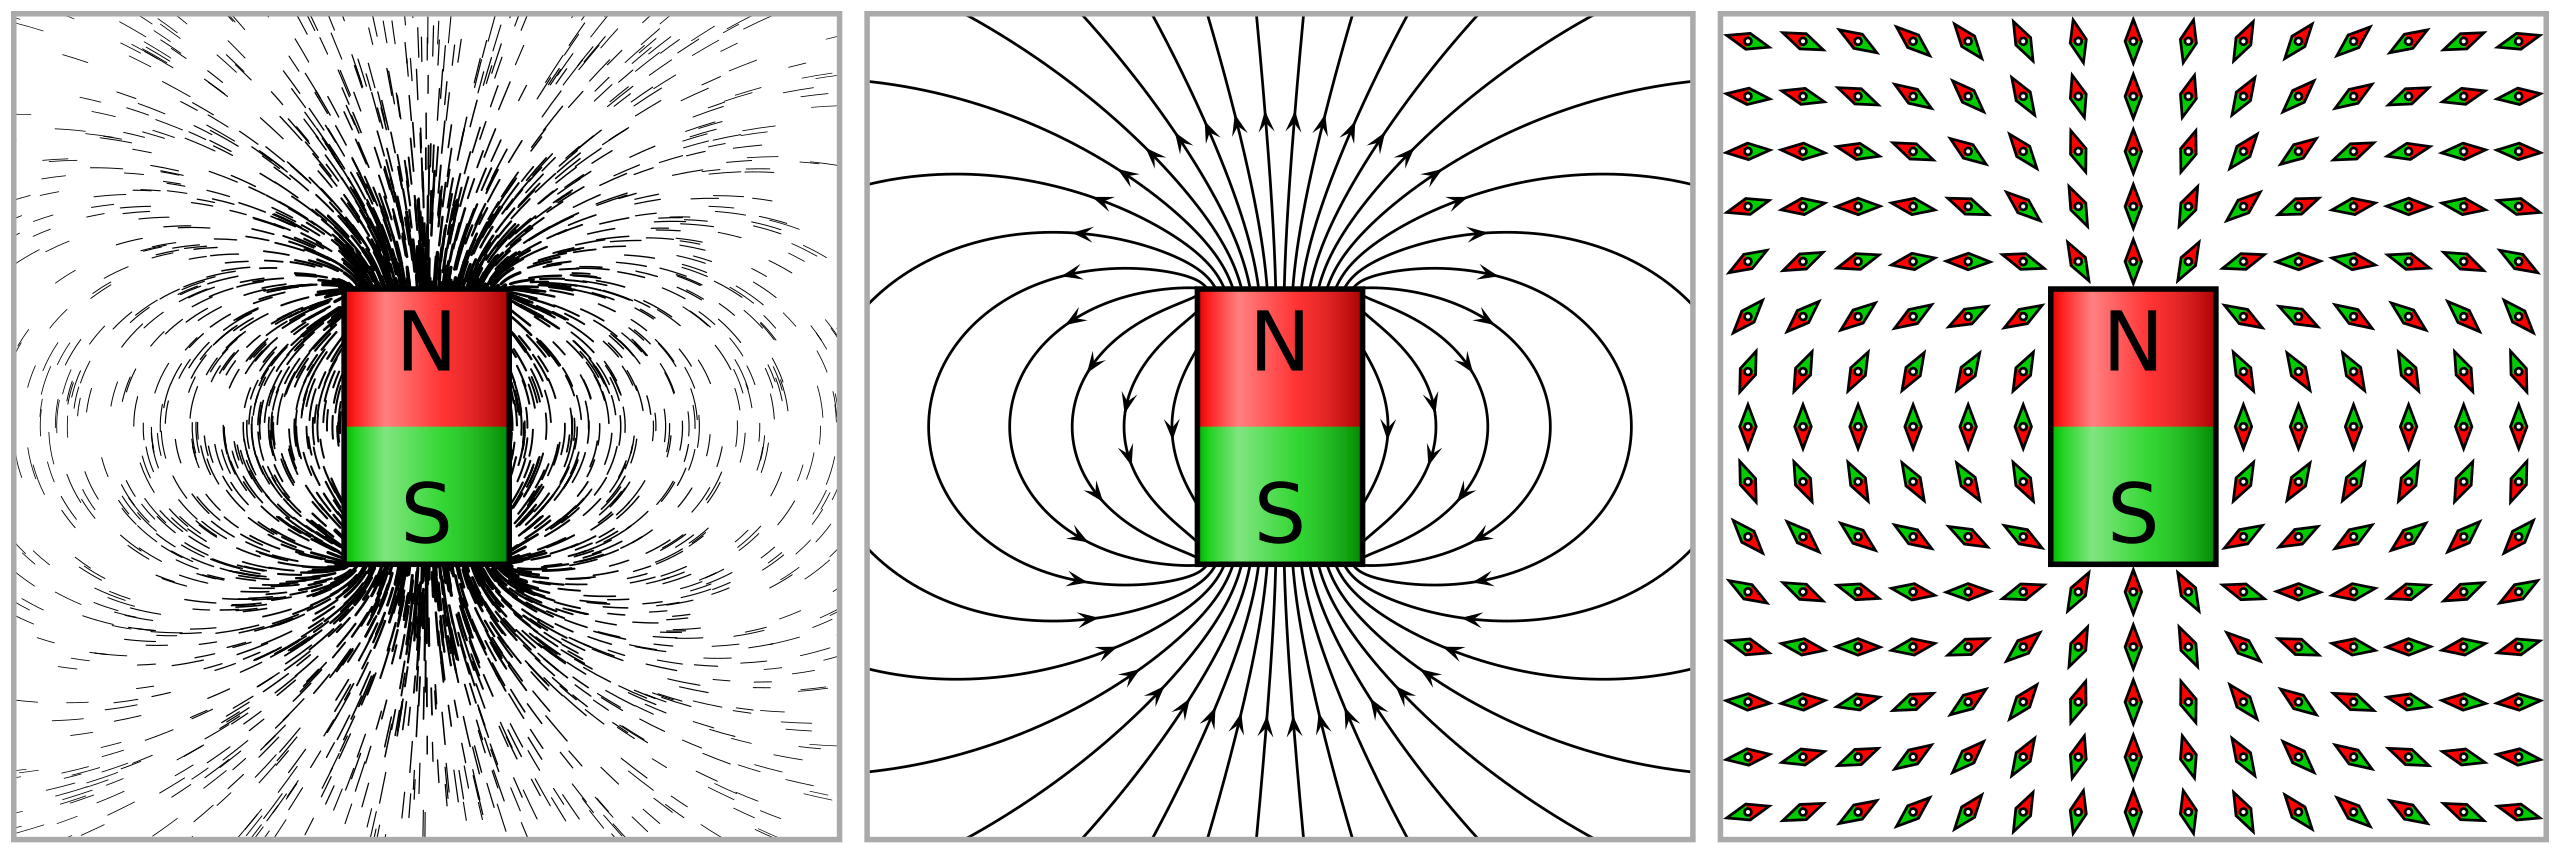
\includegraphics[width=0.5\linewidth]{figures/magnetic_field.png}}\\*
		\vfill
		%% CONTENT ENDS HERE

		{
			%%%%%%%%%%%%%%%%%%%%%%%%%%%%%%%%%%%%%%%%%%%%%%%%%%%%%%%%%%%%%%%%%%%%%%%%%%%%%%%%
			%%%%%%%%%%%%%%%%%%%%%%%%%% DO NOT MODIFY THE TABLE BELOW %%%%%%%%%%%%%%%%%%%%%%%
			%%%%%%%%%%%%%%%%%%%%%%%%%%%%%%%%%%%%%%%%%%%%%%%%%%%%%%%%%%%%%%%%%%%%%%%%%%%%%%%%
			\begin{tabular*}{16cm}{p{7.59cm} p{7.58cm}}
				\small Candidate:					&	\small Professor:\\*[10pt]
				\small\textbf{\textsc{\Author}}		&	\small\textbf{\textsc{\Professor}}\\*[10pt]
				\footnotesize  Branch : ISC	&	\footnotesize  \textbf{In collaboration with:}  \\*[10pt]
				\footnotesize  {} & \footnotesize  Thesis subject to an internship agreement: \Convention\\*[20pt]
				\footnotesize  {} & \footnotesize  Work subject to confidentiality agreement: \Confidentiel\\*[10pt]
			\end{tabular*}\\*[1.9cm]
		}

	\end{center}
\end{spacing}
